%!TEX root = ../main.tex
\chapter{Implementácia aplikácie}


\section{Dôležité triedy a ich popis}
\subsection{Klient}
\subsubsection{Komunikácia s online API}
Obycajne nic pomocou JSON a kopou phpecka a parsovanie. A vlastne POST, GET a parser.
\subsubsection{Konverzia JSON}
Ale vlastne toto je o tom praseri.
\subsection{Server}
\subsubsection{Cron}
Ktovie ci bude...a ci tu bude co opisovat

\lstset{language=Java}          % Set your language (you can change the language for each code-block optionally)

\begin{lstlisting}[frame=single]  % Start your code-block
for i:=maxint to 0 do
begin
{ do nothing }
end;
\end{lstlisting}

\section{QR kódy}
\subsection{Generovanie}
Generuje to jedna kniznica, ktora bola upravena pre codeigniter a ta bola upravená pre potreby projektu. Kedze kniznica nebola pripravená na upravu vygenerovaných obrázkov, tak boli upravene jej metody.
\subsection{Čítanie}
Specialna aktivita neviem co sem pisat okrem toho


\section{Bluetooth}
Komunikuju pomocou threadov. Aktivita v ktorej sa da vybrat zariadenie na spárovanie.

\section{Mapy}
V jednom z fragmentom, je použitá mapa. Tento komponent z 

\section{Synchronizácia súborov}

\section{Zisťovanie aktuálnej polohy}
Na zisťovanie aktuálnej polohy slúži service, ktorý sa snaží nájsť aktuálnu polohu pomocou GPS senzora poprípade internetovej siete, ku ktorej je pripojený. Trieda GPSTracker implementuje listener OnLocationChanged, pomocou ktorého je trieda notifikovaná o zmene polohy. Možnosť


\section{Databáza}
Databáza MySQL, ktorú aplikácia využíva, komunikuje s Code Igniter frameworkom. Ten pracuje s jednotlivými dátami z databáz pomocou triedy Active Record.


\section{Tvorba herného prostredia}
Vytvorena kopa MVC, kde vsetko dedi od AdminController a ten od MyControoler. Admin zarucuje vstup do sekcie iba prihlasenym a MyControler zasa základnu prácu s databázov.










\paragraph{}
Lorem ipsum 
\begin{figure}[h]
  \centering
  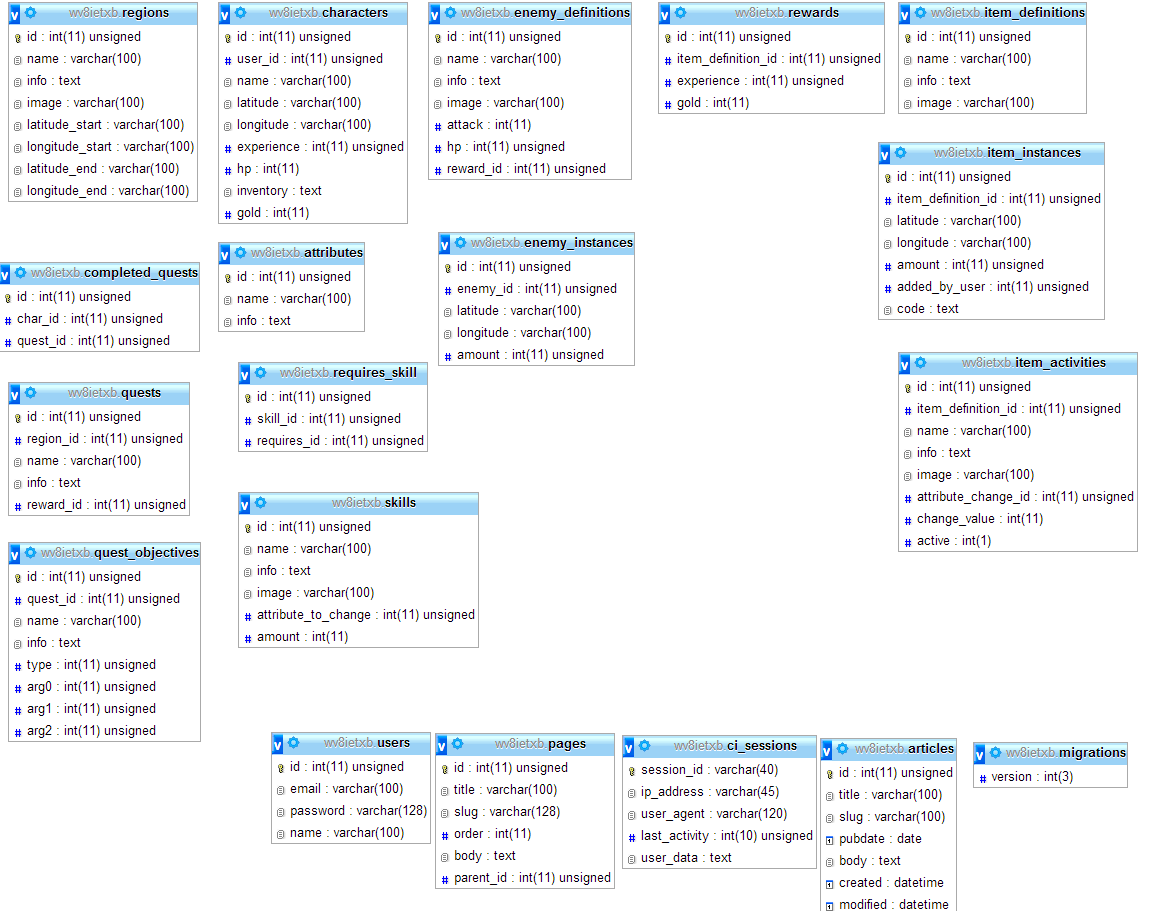
\includegraphics[height=10cm]{mainmatter/imgs/dbtemp.png}
  \caption{Temp návrh db}
  \label{fig:comenius}
\end{figure}
